\documentclass[./../../paper.tex]{subfiles}
\graphicspath{{\subfix{./../../figures/}}}

\begin{document}


\subsection{Results}
With all the configurations in mind we compare the distribution of the dataset with the distribution drawn from samples from the distribution. The configuration which best represent the data distribution is the best candidate for the next experimental steps. For this purpose, compute we the feasibility values for the Log's cases for the whole training dataset. Additionally, we sample the same number of values using our distributional approach. We show their distributions in \autoref{fig:distributions}.


\begin{figure}
    \centering
    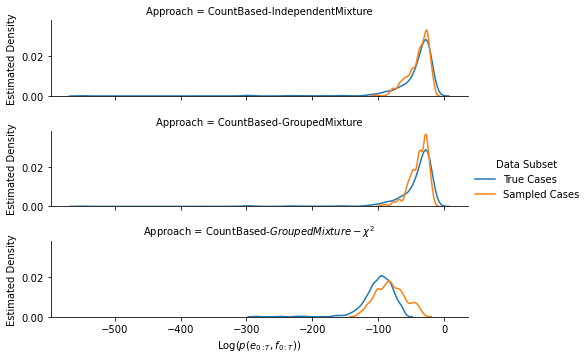
\includegraphics[width=\textwidth]{figures/results/result_distributions.png}
    \caption{The distribution of feasibility values given the approach.}
    \label{fig:distributions}
\end{figure}

As the figure is difficult to interpret, we also compute various distances using the same subsets of data. The Kolgomorov-Smirnoff Test (KST) is particularly interesting as it is a common method to compute the difference between two distributions.

\begin{table}
    \caption{The computation of various distances. Showing that the combination of Countbased Transition Estimation and the Grouped-$\chi^2$ approach consistently yields lower distances.}
    \label{tbl:distributions}
    \begin{tabular}{lllr}
     & Transition Approach & Emmision Approach & value \\
    Eval-Method &  &  &  \\
    KS-Test & CountBased & GroupedMixture & 0.411523 \\
    KS-Test & CountBased & GroupedMixture-$\chi^2$ & 0.353909 \\
    KS-Test & CountBased & IndependentMixture & 0.419753 \\
    L2 & CountBased & GroupedMixture & 0.000004 \\
    L2 & CountBased & GroupedMixture-$\chi^2$ & 0.000000 \\
    L2 & CountBased & IndependentMixture & 0.000004 \\
    L1 & CountBased & GroupedMixture & 0.000033 \\
    L1 & CountBased & GroupedMixture-$\chi^2$ & 0.000000 \\
    L1 & CountBased & IndependentMixture & 0.000031 \\
    Correlation & CountBased & GroupedMixture & 1.004166 \\
    Correlation & CountBased & GroupedMixture-$\chi^2$ & 1.004104 \\
    Correlation & CountBased & IndependentMixture & 1.010678 \\
    \end{tabular}
\end{table}

\autoref{tbl:distributions} shows that the third approach yields lower distances accross all distance methods employed.

\subsection{Discussion}
As the best configuration seems to be the \attention{CountBased-Grouped-$\chi^2$} approach, we continue with this configuration for the subsequent experiments.

However, it is important to stress that the proposed way of estimating the data distribution is one of many. The markovian approach explicitly removes the effect of past and future states. It is needless to say, a process step does not have to depend on its immediate previous state. A process outcome may be influenced by all past or future events. For instance, if one has to approve a loan in a second stage, one might be more inclined to approve something that a trusted employee already approved. Likewise, one might apply more scrutiny, knowing that a certain supervisor is going to approve the third stage.

Furthermore, this approach assumes strictly sequential processes. If the sequence has events running in parallel, we also have to record in greater detail which event has triggered a subsequent event in a given sequence. Often this knowledge is not even available.

\attention{Mention to Discuss issue with underflow}



\end{document}